\chapter{Developing a coded solution}
\section{Prototype 1 \parencite{visualstudio}}
\subsection{Login code} 
\begin{figure}[H]
    \centering
    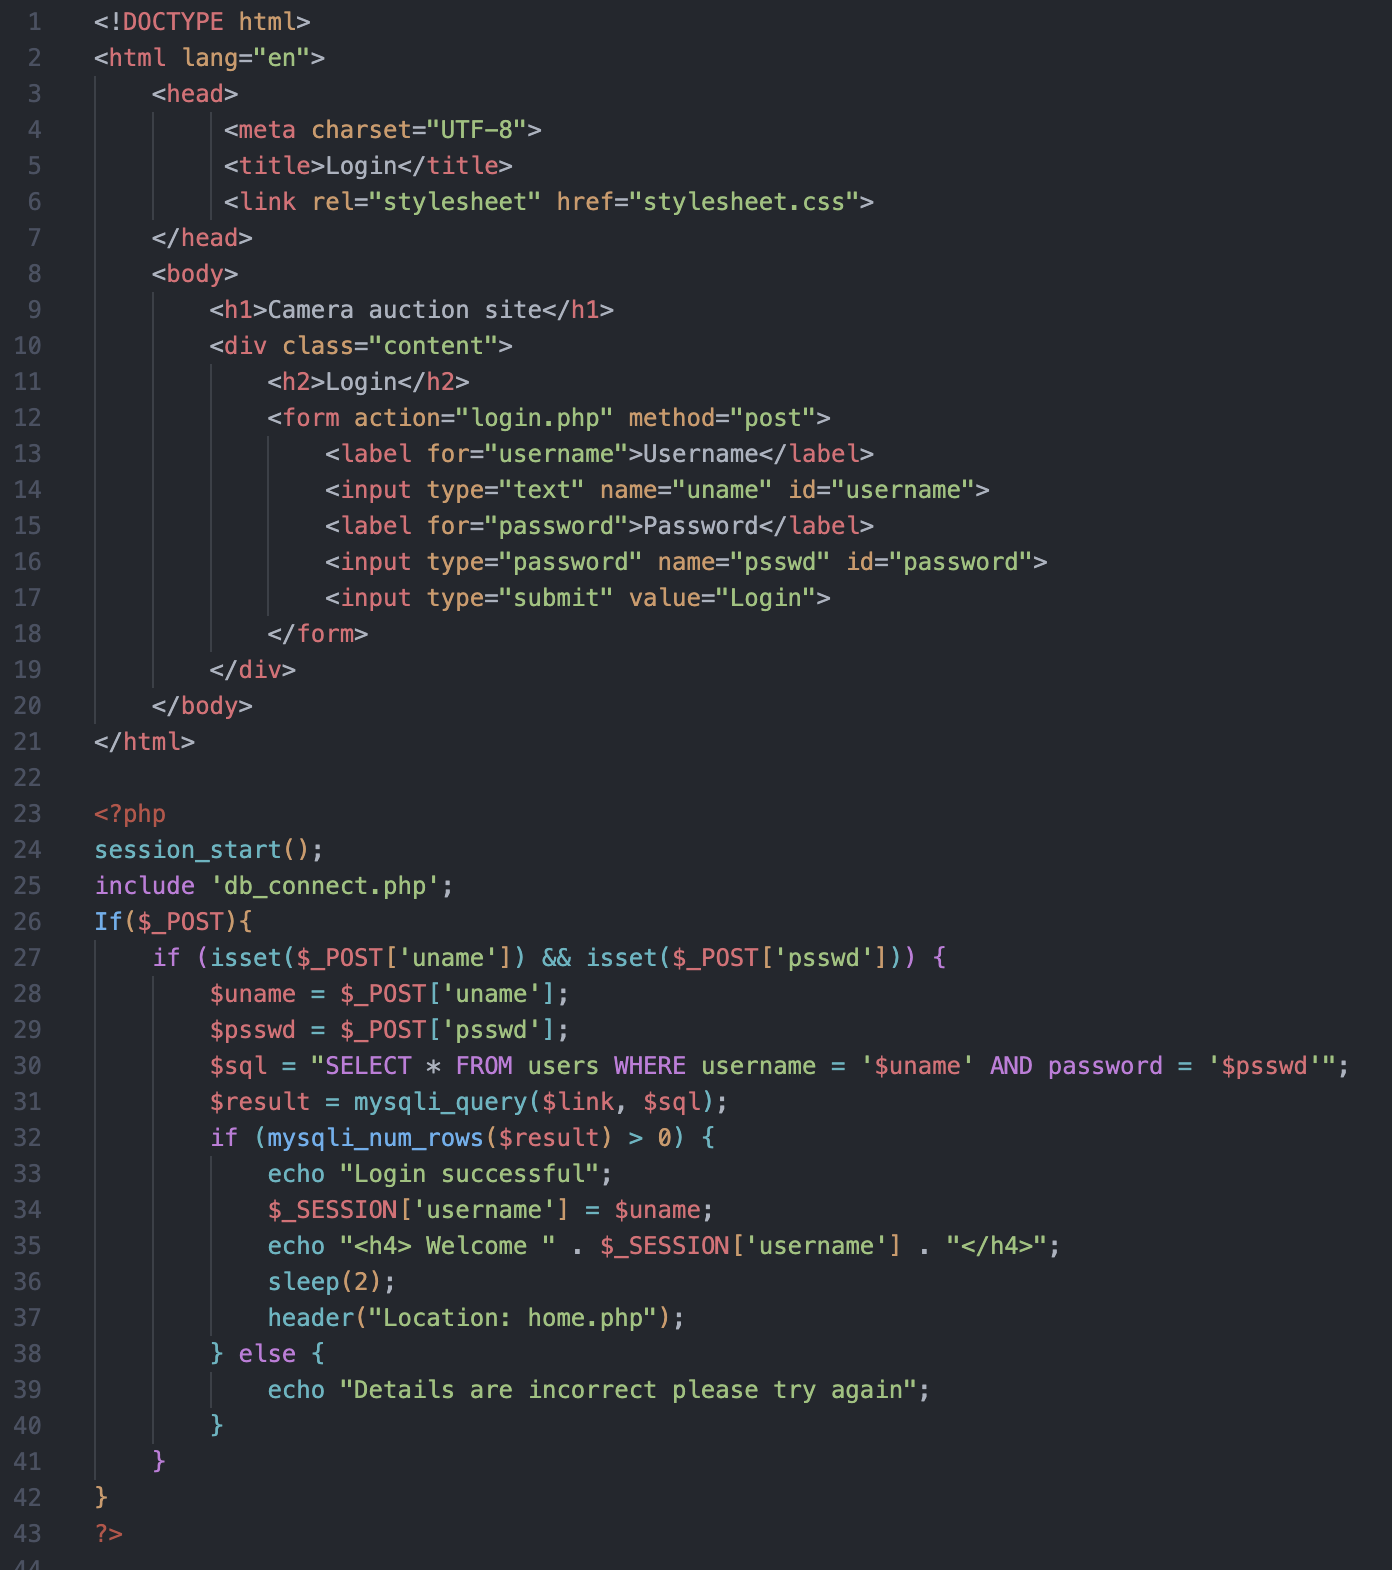
\includegraphics[scale=0.5]{ch3_developing/proto1/pro1_login.png}
    \caption{Prototype 1 login PHP code}
    \label{fig:pro1_login}
\end{figure}
The code comprises of two parts, the HTML and the PHP. The HTML primarily creates form that the user will use to log into the webpage. The PHP code first creates a session which allows variables to be stored whilst the website is running and for those variables to be transferred across pages. The database hosted on the server is also connected through use of another PHP so that it can be accessed through the code. The username and password that the user entered are then collected with the if statement ensuring that they both have text within them. Providing this is the case, the data is assigned to variables before being compiled into the SQL statement. The query is then processed with the results being stored within the results variable. The if statement checks to see if any users with the same username and password are returned, if a result is returned then we know that the user’s login details are correct else there must be an issue. If the details are correct then the user is given a success message, the username is stored in a session variable which means it can be accessed elsewhere on the site. A welcome message is presented for 2 seconds before the user is forwarded onto the home page. 

\subsection{Sign-up page}
\begin{figure}[H]
    \centering
    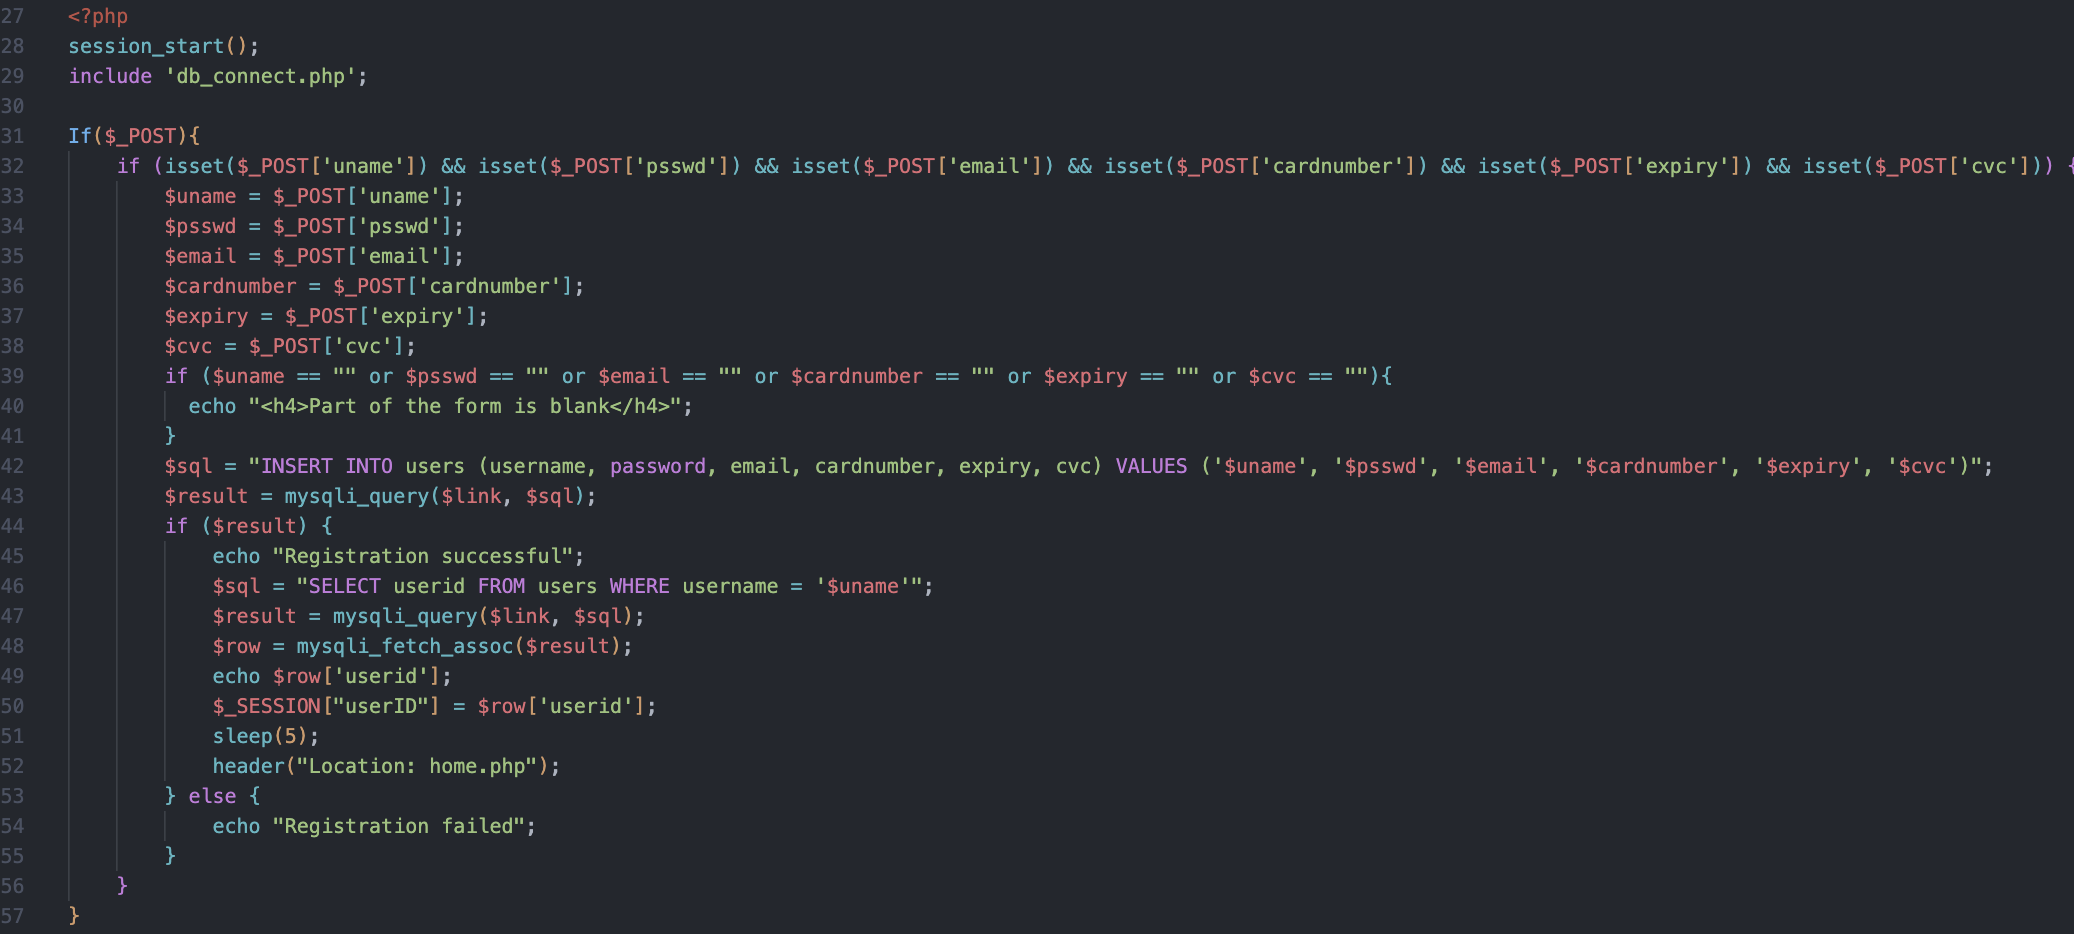
\includegraphics[scale=0.4]{ch3_developing/proto1/pro1_register.png}
    \caption{Prototype 1 sign-up PHP code}
    \label{fig:pro1_register}
\end{figure}
Similar to the login page, HTML code defines the form that the user can use, and the PHP code starts by creating a session and connecting to the database. The code will then collect the data that the user entered from the form and assign it to PHP variables. Those variables are then check in order to ensure that they contain data with an error message being returned if not. If none of the forms are blank, then the program will insert the information into the database through the SQL query. If a result is returned, then we know that it has gone through successful. The database itself ensures that the information that is being sent is unique so if an error is returned then we know there is an issue with registration which is accounted for with the else statement. If there is not an error then the users new userid is fetched through a second SQL query with the userid being assigned to a session variable. The user is then forwarded to the home page. 
\subsection{Creating a listing}
 \begin{figure}[H]
     \centering
     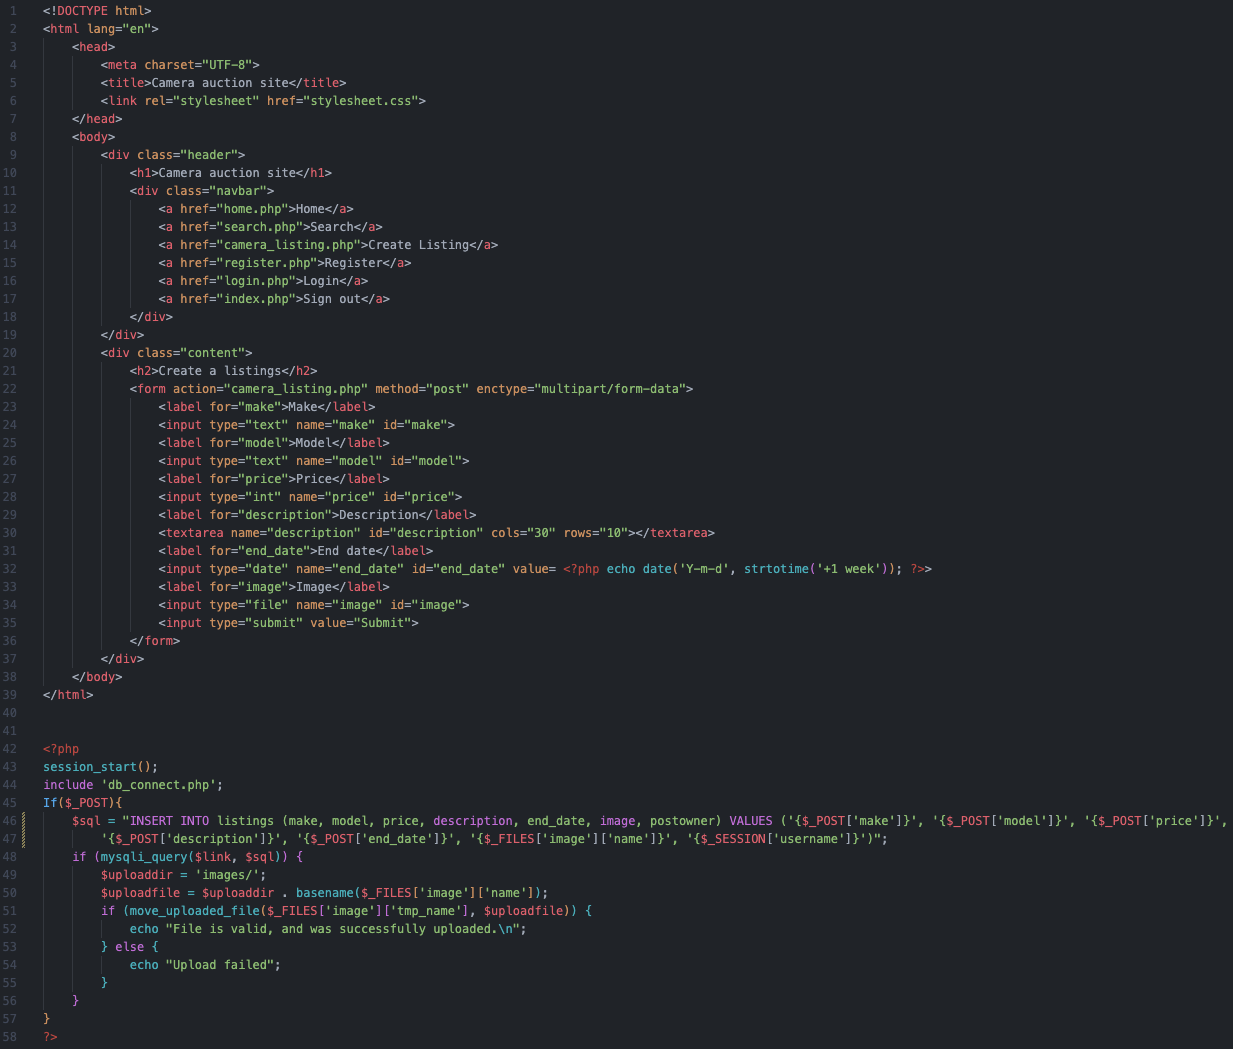
\includegraphics[scale=0.3]{ch3_developing/proto1/pro1_cameralisting.png}
     \caption{Prototype 1 PHP and HTML to create a listing}
     \label{fig:pro1_create}
 \end{figure}
The HTML takes the same format on the create a listing page, it once again consists of a large form that allows the user to add all the information that they need to in order to create the best listing. The most notable exception to the norm is that the calendar on the page is also controlled by PHP in order to by default be set to a week from the date that the user is using the website. The main PHP code first works to compile the SQL statement with the values being gathered directly through post since the variables are only needed just this one. The statement is then executed with the successful execution being the parameter for the if statement which contains the image upload code. The image upload works through adding the images to the directory in which the website files are stored and then moving the uploaded file into the right directory. Each stage is accompanied by error messages in case something was not to work.
\subsection{Search for a listing}
 \begin{figure}[H]
     \centering
     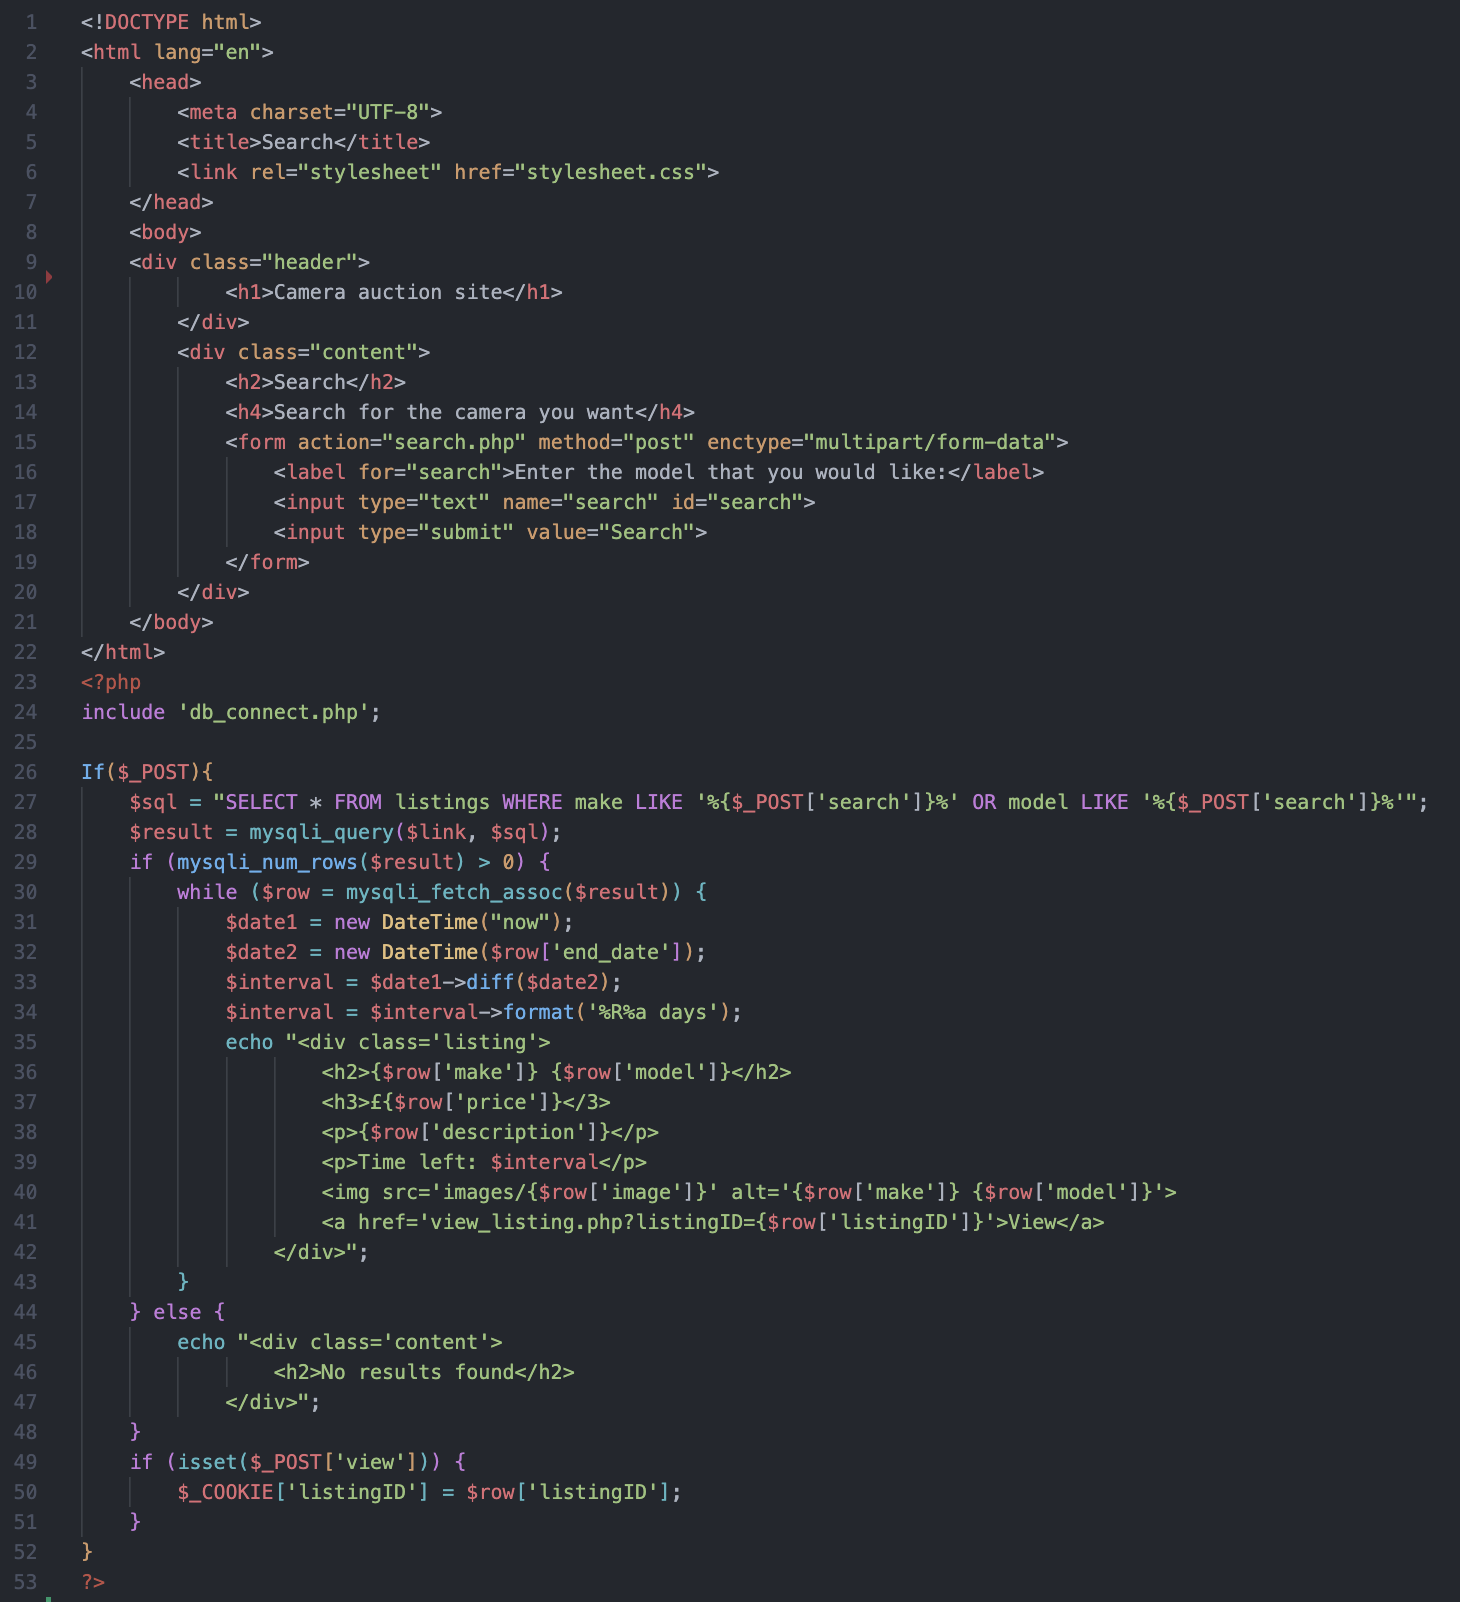
\includegraphics[scale=0.5]{ch3_developing/proto1/pro1_search.png}
     \caption{Prototype 1 PHP and HTML code for searching for a listing}
     \label{fig:pro1_search}
 \end{figure}
The search PHP code will first use the LIKE command word in SQL to find results that are close to the search term which not requiring the user to be exact. An if statement ensures that listings are returned and if not, an error is passed to the end user. If results are returned, then each of the listings will be outputting in a format defined in the echo. One notable part are the lines of PHP which calculate an interval between the end and current date and output that number in days, currently this is displayed with a plus in front. When the user press’s view, the listings listingid is cookied in order to ensure that the full view page can be retrieved. 

\subsection{View a listing}
\begin{figure}[H]
    \centering
    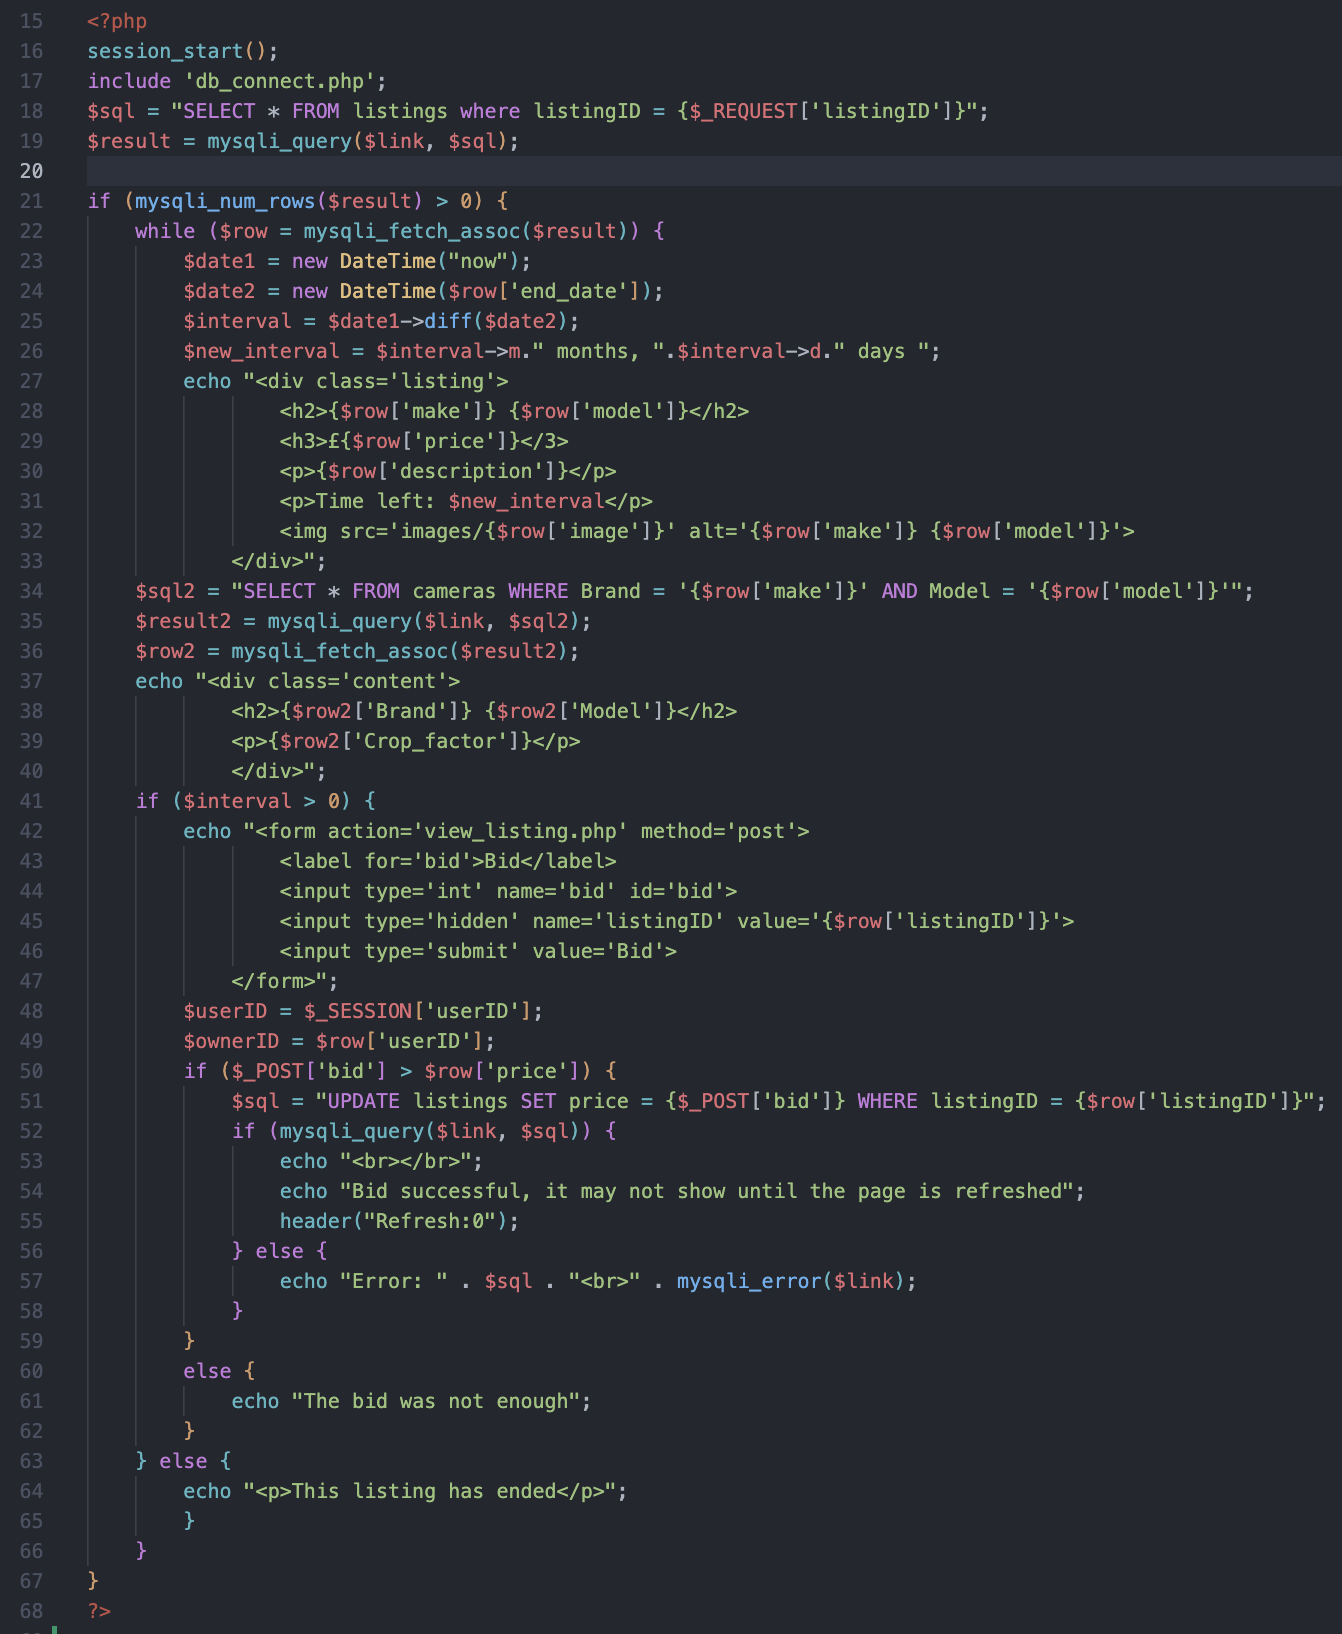
\includegraphics[scale=0.5]{ch3_developing/proto1/pro1_view.png}
    \caption{Prototype 1 PHP algorithm for viewing and bidding on a listing}
    \label{fig:pro1_view}
\end{figure}
The code will first gather all the information about a listing through a simple SQL statement that gets the listingid from the cookie that was created. The if statement that follows ensures that if information is returned from the query the rest proceeds but if not, the user is notified that their listing has ended.  The user is then shown all the specifics of their listing before the statistics of their camera which is pulled from a separate information database. The box allows the user to enter a bid where the price and current bid are compared. If the bid is greater than the updated price is sent to the database and page is refreshed. If the bid is not high enough then the user is notified and told to try again.

\subsection{Testing}
\begin{center}
\begin{longtable}{|P{17mm}|P{17mm}|P{16mm}|P{17mm}|P{40mm}|P{21.5mm}|}
  \hline
  \textbf{Test} & \textbf{Type} & \textbf{Expected result} & \textbf{Actual result} & \textbf{Test evidence} & \textbf{Changes for prototype 2}\\
  \hline
  \endfirsthead
  \hline
  \endhead
  \hline 

  \endfoot
  \endlastfoot

Incorrect login details are entered & Erroneous & Error message saying
details are wrong & Pass -- As expected &
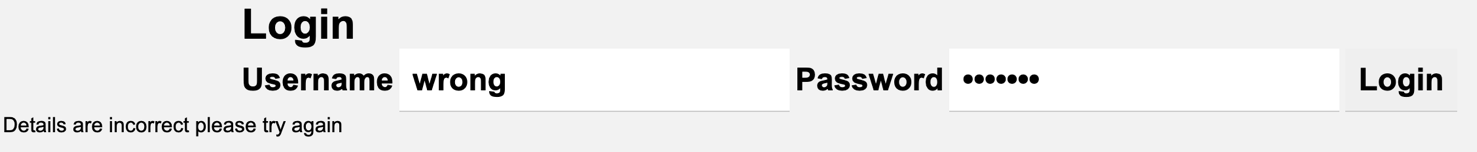
\includegraphics[width=38mm]{ch3_developing/proto1/media/image2.png}
& No changes \\ \hline
Correct login details & Normal & Welcome message and forward to home
page & Fail -- No welcome message, straight to home page &
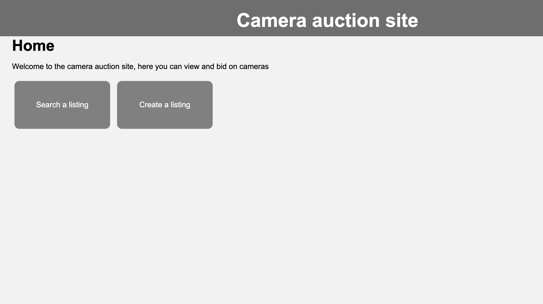
\includegraphics[width=38mm]{ch3_developing/proto1/media/image3.png}
& Assign the username to a stand-alone variable to get a welcome
message \\ \hline
Unique registration details & Normal & Forward to home page & Fail --
Not fowarded rather form resets &
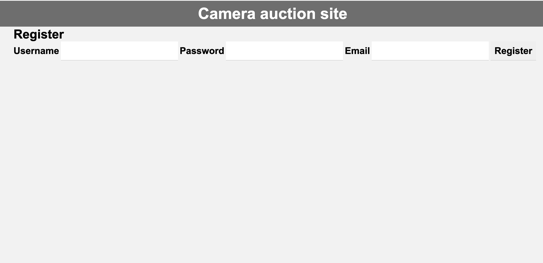
\includegraphics[width=38mm]{ch3_developing/proto1/media/image4.png}
& Add a header command to forward afterwards \\ \hline
Repeated registration details & Erroneous & Produce an error message for
the user & Fail -- No error message returned &
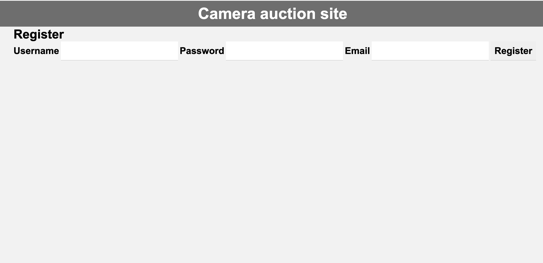
\includegraphics[width=38mm]{ch3_developing/proto1/media/image4.png}
& Add an error message \\ \hline
No details entered into registration form & Erroneous & Produce an error
message saying no details have been entered & Pass -- As expected &
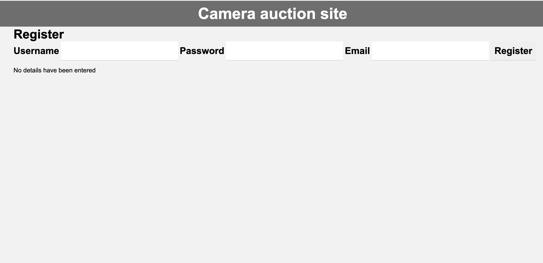
\includegraphics[width=38mm]{ch3_developing/proto1/media/image5.png}
& No changes \\ \hline
Create a listing with a non-image file & Erroneous & Produce an
incorrect file type message & Pass -- as expected &
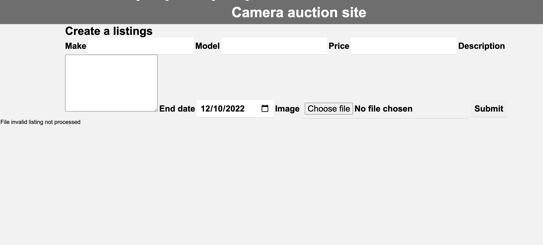
\includegraphics[width=38mm]{ch3_developing/proto1/media/image6.png}
& Change the error message to include accepted file types \\ \hline
Create a listing with no errors & Normal & Produce a message to say the
listing has been processed & Pass -- as expected &
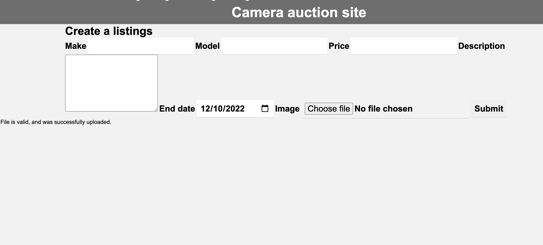
\includegraphics[width=38mm]{ch3_developing/proto1/media/image7.png}
& Move error message \\ \hline
Create a listing with 0 for a price & Erroneous & Produce an error
message that price is not valid & Fail -- Error message not produced,
and data send to database &
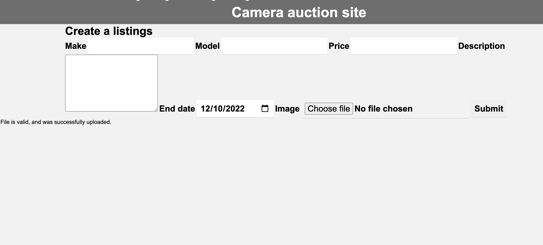
\includegraphics[width=38mm]{ch3_developing/proto1/media/image7.png}
& Only allow the price greater than 0 \\ \hline
Creating a listing with a date before today & Erroneous & Report an
error message back & Fail -- Data sent &
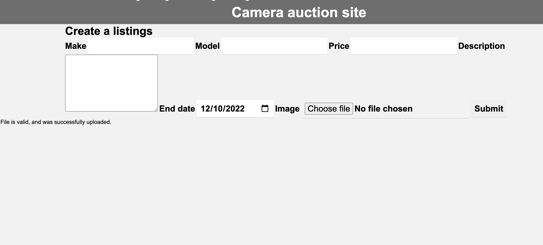
\includegraphics[width=38mm]{ch3_developing/proto1/media/image7.png}
& Compare the date with the current one and don't allow before the
date \\ \hline
Create a listing with a price of 1 & Boundary & No issues with a
positive message returned & Pass -- As expected &
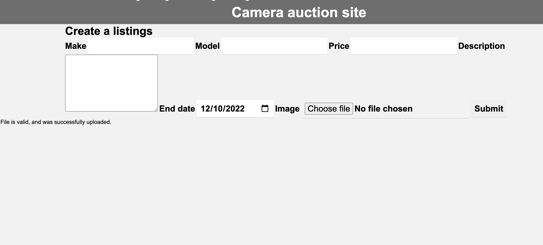
\includegraphics[width=38mm]{ch3_developing/proto1/media/image7.png}
& No changes \\ \hline
Create a listing with price as a text & Erroneous & Produce error
message that the price must be a number & Fail -- Nothing returned
include terminal error message &
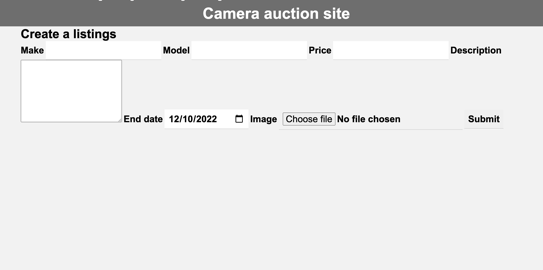
\includegraphics[width=38mm]{ch3_developing/proto1/media/image8.png}
& Add an error message detailing the problem \\ \hline
Create a listing with a super long price & Boundary & All go through as
normally should & Fail -- Nothing returned, and nothing sent to database
&
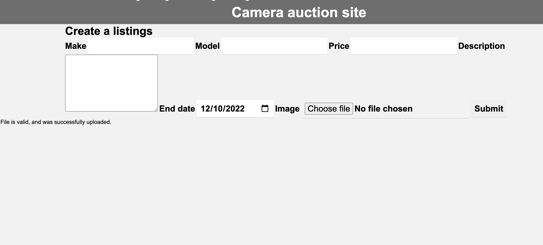
\includegraphics[width=38mm]{ch3_developing/proto1/media/image7.png}
& Increase the number limit size in the database and ensure prices are
not greater than 6 sig fig \\ \hline
Adding a price with a decimal & Normal & Price is rounded and sent to
database & Pass -- Rounding all correct &
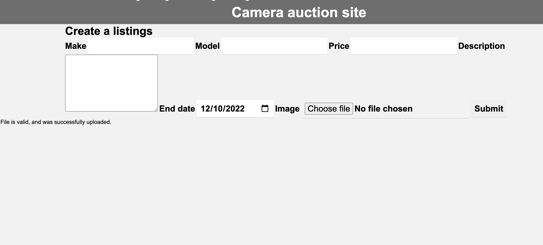
\includegraphics[width=38mm]{ch3_developing/proto1/media/image7.png}
& Adjust the data type of the column in the database to allow floats \\ \hline
Does a search box appear on the page & Normal & Text input box with
button the page & Pass -- Box appears &

\includegraphics[width=38mm]{ch3_developing/proto1/media/image10.png}
& Nothing to change \\ \hline
Do listings appear if the user enters a valid camera & Normal & Listing
appears with the image & Partial pass- Listing returned image not due to
referencing issues &

\includegraphics[width=38mm]{ch3_developing/proto1/media/image11.png}
& Move the images to be stored outside of the updated directory \\ \hline
User does not enter any text but still searches & Boundary & No listings
are returned, and an error is given & Fail -- All listings are returned
&
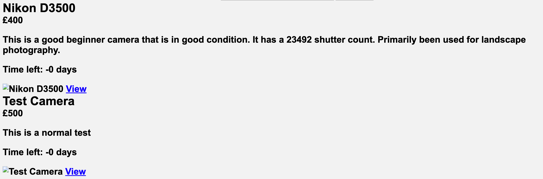
\includegraphics[width=38mm]{ch3_developing/proto1/media/image12.png}
& Check the user has entered text before sending the query \\ \hline

    \caption{Prototype 1 testing table}
\label{tab:proto1_testing}
\end{longtable}
\end{center}

\subsection{Plans for prototype 2}
For prototype 2, I’m aiming to add the collection of card details to the website when the user registers. This itself will also mean that more verification has to be added to the program. Since the tests also failed with the price recommendation page since the page was not built. The next prototype will aim to fix this by building a price recommendation as previously outlined. The button will also be added to the homepage. Currently, only basic camera information is fetched from the database on the camera due to the time it would have taken to process all the information. With prototype 2, I am aiming to add the full camera information that is fetched from the database. The aim is also to add and fix verification algorithms on all the pages. 
